\documentclass[twoside,UTF8]{EPURapport}
%\usepackage{listings}

%\renewcommand{\lstlistlistingname}{Liste des codes}
%\renewcommand{\lstlistingname}{Code}

%\addextratables{%
%	\lstlistoflistings
%}

%\swapAuthorsAndSupervisors
\usepackage{float}


\thedocument{Rapport de projet}{Développement d'un site de vente et de gestion pour la Kfet de Polytech}{Site web Kfet}

\grade{Département Informatique\\ 5\ieme{} année\\ 2011 - 2012}

\authors{%
	\category{Étudiants}{%
		\name{Loïc CARNEY} \mail{loic.carney@etu.univ-tours.fr}
		\name{Sébastien LACROIX} \mail{sebastien.lacroix@etu.univ-tours.fr}
	}
	\details{DI5 2008 - 2009}
}

\supervisors{%
	\category{Encadrants}{%
		\name{Alexandre LISSY} \mail{alexandre.lissy@univ-tours.fr}
	}
	\details{Université François-Rabelais, Tours}
}

\abstracts{Description en français}
{Mots clés français}
{Description en anglais}
{Mots clés en anglais}

\begin{document}
\renewcommand{\labelitemi}{\textbullet}

\chapter{Introduction}

    \paragraph{}Dans le cadre de notre dernière année d'étude à Polytech'Tours, nous devions réaliser un projet lié aux technologies web. Nous avons décider de proposer notre propre sujet. L'un de nous ayant été trésorier à la Kfet du département Informatique de l'école, nous étions au courant que toute la gestion de la Kfet se fait sur papier et manuellement. Aucune gestion automatique n'est en place et aucune gestion des stocks n'est effectuée pour le moment. Nous avons donc proposer comme sujet : la réalisation d'un site web permettant de répondre à tous les besoins de gestion de la Kfet: en commençant par la vente jusqu'à la gestion des stocks et en passant par la gestion des dettes.

    \paragraph{}Pour réaliser le projet web, nous avons décidé d'utiliser une technologie web que nous ne connaissions pas : le  framework web Django qui est basé sur le langage interprêté Python. Le but de Django est de donner au développeur web des outils simples et rapides, en effet son slogan est "Le framework web pour les perfectionnistes sous pression".

    \paragraph{}La Kfet de Polytech est ouverte à toutes les pauses. Lors des pauses d'inter-cours elle vend des en-cas, confiseries et des boissons chaudes,et lors de la pause de midi elle sert des plats chauds. Les stocks sont donc assez conséquents et varient fortement, la problématique de la gestion des stocks est un des éléments qui nous a incité à réaliser ce projet.

    \paragraph{}Nous allons donc vous présenter tout d'abord le projet au travers du cahier des charges puis nous détaillerons le fonctionnement de chaque module mis en place.

%%%%%%%%%%%%%%%%%%%%%%%%%%%%%%%%%%%%%%%%%%%%%%%%%%%%%%%%%%%%%%%%%%%%%%%%%%%%%%%%%%%%%%%%%%%%%%%%%%%%ù
%%%%%%%%%%%%%%%%%%%%%%%%%%%%%%%%%%%%%%%%%%%%%%%%%%%%%%%%%%%%%%%%%%%%%%%%%%%%%%%%%%%%%%%%%%%%%%%%%%%%ù
%%%%%%%%%%%%%%%%%%%%%%%%%%%%%%%%%%%%%%%%%%%%%%%%%%%%%%%%%%%%%%%%%%%%%%%%%%%%%%%%%%%%%%%%%%%%%%%%%%%%ù
\chapter{Cahier des charges}
% TODO Seb

    \paragraph{}Nous allons dans cette partie définir les fonctionnalités attendues par la Kfet afin de simplifier la vie de ses membres. Nous allons pour cela décomposer les fonctionnalités par rôles de l'association. 
    \paragraph{}Nous allons donc dans un premier temps définir les fonctionnalités de gestion d'association, puis les fonctionnalités d'un kftier vendeur, enfin nous définirons les fonctionnalités proposés à un étudiant non membre de l'association.

    \section{Fonctionnalités de gestion}

        \paragraph{}Le but premier de ce projet était de remettre en place une réelle gestion au sein de la Kfet. Nous voulions ainsi permettre de suivre en détails les stocks, les ventes de la journée ou du mois, le chiffre d'affaire ...

        \subsection{Gestion des stocks}

            \paragraph{}Le manque de gestion administrative de la Kfet entraine une faiblesse majeure : presque aucune gestion des stocks n'est assurée. Cette faiblesse se ressent le plus lors du manque de pizza le midi et le mécontentement des clients qui en découle.
            \paragraph{}Nous nous proposons donc de mettre en place une gestion des stocks complète apportant les fonctionnalités suivantes :\\
            \begin{itemize}
                \item Ajout de fournisseur : Pouvoir avoir plusieurs fournisseur différents, notamment afin de pouvoir différencier les commandes ;\\
                \item Commande de produit : Pouvoir avoir une trace de la commande effectué auprès du fournisseur et ne la valider qu'une fois arrivée. Nous voulons ainsi différencier les produits en stocks, des commandes ;\\
                \item Notification de fin de stock : Recevoir une notification par mail lorsqu'un stock atteint le seuil limite afin de pouvoir réapprovisionner avant la rupture.\\
            \end{itemize}

        \subsection{Gestion des finances}

            \paragraph{}Nous voulions apporter à la Kfet des outils de gestion permettant d'avoir des informations sur les ventes, le chiffre d'affaire ... Ces outils pourrons par exemple permettre de mettre en avant des pertes trop importantes sur certains produits. Nous avons donc définis les fonctionnalités suivantes :\\

            \begin{itemize}
                \item Statistiques de ventes : afficher le chiffre d'affaire, les ventes réalisées sur une période définie ;\\
                \item Gestion des dettes : pouvoir gérer les dettes de tous les clients de façon informatique (enseignants et étudiants) et pouvoir les avertir lorsqu'un plafond est atteint.
            \end{itemize}

    \section{Fonctionnalités de vente}
        
        \paragraph{}Afin de simplifier la gestion de stock et le fonctionnement de la Kfet nous avons voulu proposer des fonctionnalités de ventes. 

        \paragraph{}La partie vente se décompose en deux type : les commande de menus le midi, et les ventes individuelles.

        \subsection{Gestion des commandes}
            \paragraph{}Les fonctionnalités permettant de gérer les commandes vont permettre de supprimer tous le système complexe et non productif des papier de commande. Nous proposons donc les fonctions suivantes :
        
            \begin{itemize}
                \item Gestion de commandes : validation, paiement, annulation ;\\                
                \item Historique permettant un calcul de chiffre d'affaire.
            \end{itemize}

        \subsection{Ventes}
            \paragraph{}Afin de pouvoir avoir une gestion des stocks complète il faut qu'une chaque vente soit enregistrée de manière informatique. Pour cela nous proposons de mettre en place une interface facilement adaptable à un appareil tactile permettant de vendre à l'unité ou en lot et permettant de mettre la vente en dette. Une gestion avancée de celles-ci pourra de plus être mise en place permettant d'annuler la vente en cas d'erreur par exemple.

    \section{Fonctionnalités utilisateur}

        \paragraph{}Nous avons voulu proposer des fonctionnalités simplifiant la gestion de la Kfet, mais nous voulons aussi proposer des fonctionnalités intéressantes aux clients.

        \paragraph{}Nous proposons pour cela de mettre en place un site de e-commerce permettant de réaliser n'importe qu'elle commande en avance. Cela évitera, par exemple, dans le cas de la vente de pizza la cohue au comptoir due au nombre limité de commande.

        \paragraph{}Un compte utilisateur permettra de plus de pouvoir consulter sa dette, voire de la régler par carte bleue ou paypal.
        


%%%%%%%%%%%%%%%%%%%%%%%%%%%%%%%%%%%%%%%%%%%%%%%%%%%%%%%%%%%%%%%%%%%%%%%%%%%%%%%%%%%%%%%%%%%%%%%%%%%%ù
%%%%%%%%%%%%%%%%%%%%%%%%%%%%%%%%%%%%%%%%%%%%%%%%%%%%%%%%%%%%%%%%%%%%%%%%%%%%%%%%%%%%%%%%%%%%%%%%%%%%ù
%%%%%%%%%%%%%%%%%%%%%%%%%%%%%%%%%%%%%%%%%%%%%%%%%%%%%%%%%%%%%%%%%%%%%%%%%%%%%%%%%%%%%%%%%%%%%%%%%%%%ù
\chapter{Le framework Django}
% TODO Loic

%%%%%%%%%%%%%%%%%%%%%%%%%%%%%%%%%%%%%%%%%%%%%%%%%%%%%%%%%%%%%%%%%%%%%%%%%%%%%%%%%%%%%%%%%%%%%%%%%%%%ù
%%%%%%%%%%%%%%%%%%%%%%%%%%%%%%%%%%%%%%%%%%%%%%%%%%%%%%%%%%%%%%%%%%%%%%%%%%%%%%%%%%%%%%%%%%%%%%%%%%%%ù
%%%%%%%%%%%%%%%%%%%%%%%%%%%%%%%%%%%%%%%%%%%%%%%%%%%%%%%%%%%%%%%%%%%%%%%%%%%%%%%%%%%%%%%%%%%%%%%%%%%%ù
\chapter{Module Compte}
% TODO Seb

%%%%%%%%%%%%%%%%%%%%%%%%%%%%%%%%%%%%%%%%%%%%%%%%%%%%%%%%%%%%%%%%%%%%%%%%%%%%%%%%%%%%%%%%%%%%%%%%%%%%ù
%%%%%%%%%%%%%%%%%%%%%%%%%%%%%%%%%%%%%%%%%%%%%%%%%%%%%%%%%%%%%%%%%%%%%%%%%%%%%%%%%%%%%%%%%%%%%%%%%%%%ù
%%%%%%%%%%%%%%%%%%%%%%%%%%%%%%%%%%%%%%%%%%%%%%%%%%%%%%%%%%%%%%%%%%%%%%%%%%%%%%%%%%%%%%%%%%%%%%%%%%%%ù
\chapter{Module Commandes}
% TODO Seb

%%%%%%%%%%%%%%%%%%%%%%%%%%%%%%%%%%%%%%%%%%%%%%%%%%%%%%%%%%%%%%%%%%%%%%%%%%%%%%%%%%%%%%%%%%%%%%%%%%%%ù
%%%%%%%%%%%%%%%%%%%%%%%%%%%%%%%%%%%%%%%%%%%%%%%%%%%%%%%%%%%%%%%%%%%%%%%%%%%%%%%%%%%%%%%%%%%%%%%%%%%%ù
%%%%%%%%%%%%%%%%%%%%%%%%%%%%%%%%%%%%%%%%%%%%%%%%%%%%%%%%%%%%%%%%%%%%%%%%%%%%%%%%%%%%%%%%%%%%%%%%%%%%ù
\chapter{Module Gestion Stocks}
% TODO Loïc

%%%%%%%%%%%%%%%%%%%%%%%%%%%%%%%%%%%%%%%%%%%%%%%%%%%%%%%%%%%%%%%%%%%%%%%%%%%%%%%%%%%%%%%%%%%%%%%%%%%%ù
%%%%%%%%%%%%%%%%%%%%%%%%%%%%%%%%%%%%%%%%%%%%%%%%%%%%%%%%%%%%%%%%%%%%%%%%%%%%%%%%%%%%%%%%%%%%%%%%%%%%ù
%%%%%%%%%%%%%%%%%%%%%%%%%%%%%%%%%%%%%%%%%%%%%%%%%%%%%%%%%%%%%%%%%%%%%%%%%%%%%%%%%%%%%%%%%%%%%%%%%%%%ù
\chapter{Module Ventes}
% TODO Seb

    \paragraph{}Nous allons vous présenter dans cette partie le module de ventes du site web. Voici tout d'abord une capture d'écran de la page de ventes vue par un kftier.
    \begin{center}
        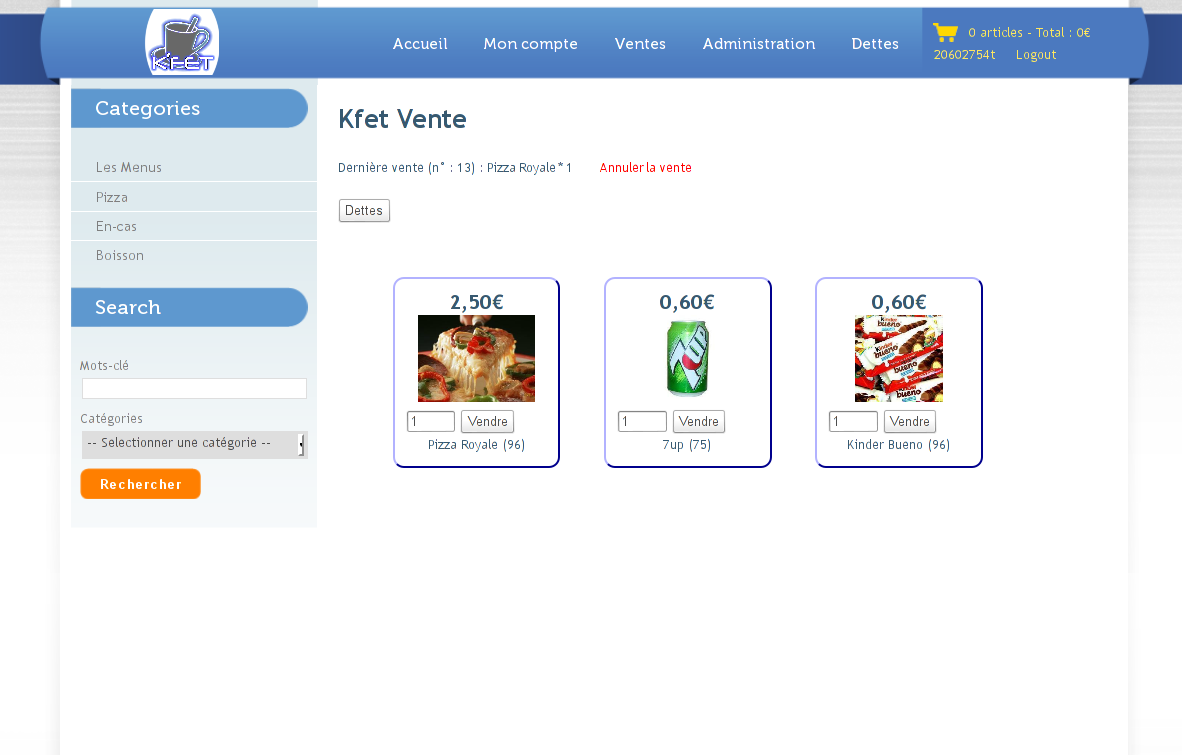
\includegraphics[width=1\linewidth]{logos/ventes.png}
    \end{center}
    \paragraph{}Nous allons dans un premier temps définir les fonctionnalités disponible dans la page, puis nous détaillerons le fonctionnement de celles-ci.

    \section{Détail des fonctionnalités}

        \paragraph{}Lorsque un kftier veut vendre un produit il se rend sur cette page. La page indique plusieurs informations : \\
            \begin{itemize}
                \item Les produits avec pour chaque produit : son prix, sa quantité restante entre parenthèse, une image le représentant ;\\
                \item Une indication "épuisé" lorsqu'un produit n'est plus disponible ;\\
                \item La dernière vente effectuée et la possibilité d'annuler celle-ci en cas d'erreur ;\\
                \item Une liste, pouvant être dissimuler, permettant de sélectionner la personne voulant payer en dette.\\
            \end{itemize}

    \section{Fonctionnement du module}

        \subsection{Modèle de base de donnée}

            \paragraph{}Les attributs de la table vente, permettant de stocker les informations de vente sont les suivants :\\
            \begin{itemize}
                \item produit\_id : identifiant du produit venu ;\\
                \item date : la date de la vente ;\\
                \item quantite : la quantité vendue ;\\
                \item user\_id : identifiant de l'utilisateur en cas de vente avec dette.
            \end{itemize}

        \subsection{Fonction du contrôleur}

            \paragraph{index}Cette fonction permet d'afficher l'index des ventes. Elle récupère tous les produits à afficher et vérifie leurs disponibilités. Elle récupère de plus la dernière vente effectuée.

            \paragraph{produit\_vente}Cette fonction permet de réaliser une vente. Elle vérifie la présence ou non de la sélection d'une personne et effectue la vente. Dans le cas où une personne est sélectionnée elle augmente la dette de celle-ci du montant de la vente. Les stocks sont de plus déduit en fonction de la quantité sélectionnée.
            \paragraph{annuler\_vente}Cette fonction annule la dernière vente effectuée en supprimant l'entrée de la base de donnée. Le stock est réapprovisionner et si une dette a été ajoutée elle est annulée.

        \subsection{Fonction du template}

            \paragraph{}Le template réalisant l'affichage de la page est formée de plusieurs formulaires et ayant chacun leurs boutons de validation.

            \paragraph{}Du javascript a été nécessaire pour la sélection du nom de la personne à ajouter en dette, en effet une seule sélection est répercutée sur tous les formulaires de la page.

            \paragraph{}Enfin une pagination est mise en place à l'aide de Django et définie à la fois dans le contrôleur et la vue.


%%%%%%%%%%%%%%%%%%%%%%%%%%%%%%%%%%%%%%%%%%%%%%%%%%%%%%%%%%%%%%%%%%%%%%%%%%%%%%%%%%%%%%%%%%%%%%%%%%%%ù
%%%%%%%%%%%%%%%%%%%%%%%%%%%%%%%%%%%%%%%%%%%%%%%%%%%%%%%%%%%%%%%%%%%%%%%%%%%%%%%%%%%%%%%%%%%%%%%%%%%%ù
%%%%%%%%%%%%%%%%%%%%%%%%%%%%%%%%%%%%%%%%%%%%%%%%%%%%%%%%%%%%%%%%%%%%%%%%%%%%%%%%%%%%%%%%%%%%%%%%%%%%ù
\chapter{Module Administration}
% TODO Loic

%%%%%%%%%%%%%%%%%%%%%%%%%%%%%%%%%%%%%%%%%%%%%%%%%%%%%%%%%%%%%%%%%%%%%%%%%%%%%%%%%%%%%%%%%%%%%%%%%%%%ù
%%%%%%%%%%%%%%%%%%%%%%%%%%%%%%%%%%%%%%%%%%%%%%%%%%%%%%%%%%%%%%%%%%%%%%%%%%%%%%%%%%%%%%%%%%%%%%%%%%%%ù
%%%%%%%%%%%%%%%%%%%%%%%%%%%%%%%%%%%%%%%%%%%%%%%%%%%%%%%%%%%%%%%%%%%%%%%%%%%%%%%%%%%%%%%%%%%%%%%%%%%%ù
\chapter{Module dettes}
% TODO Loïc

%%%%%%%%%%%%%%%%%%%%%%%%%%%%%%%%%%%%%%%%%%%%%%%%%%%%%%%%%%%%%%%%%%%%%%%%%%%%%%%%%%%%%%%%%%%%%%%%%%%%ù
%%%%%%%%%%%%%%%%%%%%%%%%%%%%%%%%%%%%%%%%%%%%%%%%%%%%%%%%%%%%%%%%%%%%%%%%%%%%%%%%%%%%%%%%%%%%%%%%%%%%ù
%%%%%%%%%%%%%%%%%%%%%%%%%%%%%%%%%%%%%%%%%%%%%%%%%%%%%%%%%%%%%%%%%%%%%%%%%%%%%%%%%%%%%%%%%%%%%%%%%%%%ù
\chapter{Conclusion}
% TODO Loïc

%%%%%%%%%%%%%%%%%%%%%%%%%%%%%%%%%%%%%%%%%%%%%%%%%%%%%%%%%%%%%%%%%%%%%%%%%%%%%%%%%%%%%%%%%%%%%%%%%%%%ù
%%%%%%%%%%%%%%%%%%%%%%%%%%%%%%%%%%%%%%%%%%%%%%%%%%%%%%%%%%%%%%%%%%%%%%%%%%%%%%%%%%%%%%%%%%%%%%%%%%%%ù
%%%%%%%%%%%%%%%%%%%%%%%%%%%%%%%%%%%%%%%%%%%%%%%%%%%%%%%%%%%%%%%%%%%%%%%%%%%%%%%%%%%%%%%%%%%%%%%%%%%%ù
%%%%%%%%%%%%%%%%%%%%%%%%%%%%%%%%%%%%%%%%%%%%%%%%%%%%%%%%%%%%%%%%%%%%%%%%%%%%%%%%%%%%%%%%%%%%%%%%%%%%ù
%%%%%%%%%%%%%%%%%%%%%%%%%%%%%%%%%%%%%%%%%%%%%%%%%%%%%%%%%%%%%%%%%%%%%%%%%%%%%%%%%%%%%%%%%%%%%%%%%%%%ù
\annexes

\end{document}

